\documentclass{article}
\usepackage{amsmath}
\usepackage{enumitem}
\usepackage{setspace} % Add this package for line spacing
\usepackage{graphicx}
\usepackage{geometry}
\usepackage{hyperref}
\usepackage{tabularx}
\usepackage{float}

\title{Apple's Neural Processing Units (NPUs) and Neural Engine}
\author{}
\date{}

\begin{document}

% Set line spacing for the entire document
\setstretch{1.2} % Adjust to your preference (1.2 for slightly increased spacing)

% Custom title page content
\begin{titlepage}
    \centering
    {\Large \textbf{Assignment \# 2}} % Title in large bold text
    \vspace{0.1in}
		
		\vspace*{0.3in}
    
\includegraphics[width=0.3\textwidth]{./images/UetLogo.png} % Optional: add logo image
    \vspace{0.8in}
    
    {\large \textbf{Fall 2024}  \\ 
						\textbf{CSE-420 Embedded Systems}
						} % Author info
    \vspace{0.5in} 
    
    {\large \textbf{Name:} Ali Asghar \\ 
						\textbf{Registration:} 21PWCSE2059 \\
						\textbf{Section:} A \\
		} % Author info
    \vspace{0.5in}
		
    {\large Submitted to:\\ 
						\textbf{Dr.Asif Ali Khan} \\						
		} % Author info
    \vspace{0.5in}

    {\large Date:\\ 
						\textbf{7th November, 2024} \\						
		} % Author info
    \vspace{0.5in}
		
		{\large \textbf{Department of Computer Systems Engineering}\\ 
						\textbf{University of Engineering and Technology, Peshawar} \\						
		} % Author info
    %\vspace{0.5in}
		
    \vfill
\end{titlepage}

% Start the main document without a duplicate title page
\newpage % Page break after cover page

%\maketitle

\section*{Apple Neural Engine}
The Apple Neural Engine (or ANE) is a type of NPU, which stands for Neural Processing Unit. It's like a GPU, but instead of accelerating graphics an NPU accelerates neural network operations such as convolutions and matrix multiplies\cite{ANEGithub}. It was introduced with the A11 Bionic chip, and is a dedicated hardware block within Apple’s system-on-chip (SoC) designed specifically for accelerating machine learning and artificial intelligence tasks.

The ANE isn't the only NPU out there — many companies besides Apple are developing their own AI accelerator chips. Besides the Neural Engine, the most famous NPU is Google's TPU (or Tensor Processing Unit). In Figure \ref{fig:Apple_A17_Chip2} below, we can see the ANE in recently launched Apple A17 Pro Chip having 16 cores. 


\begin{figure}[H]
	\centering
		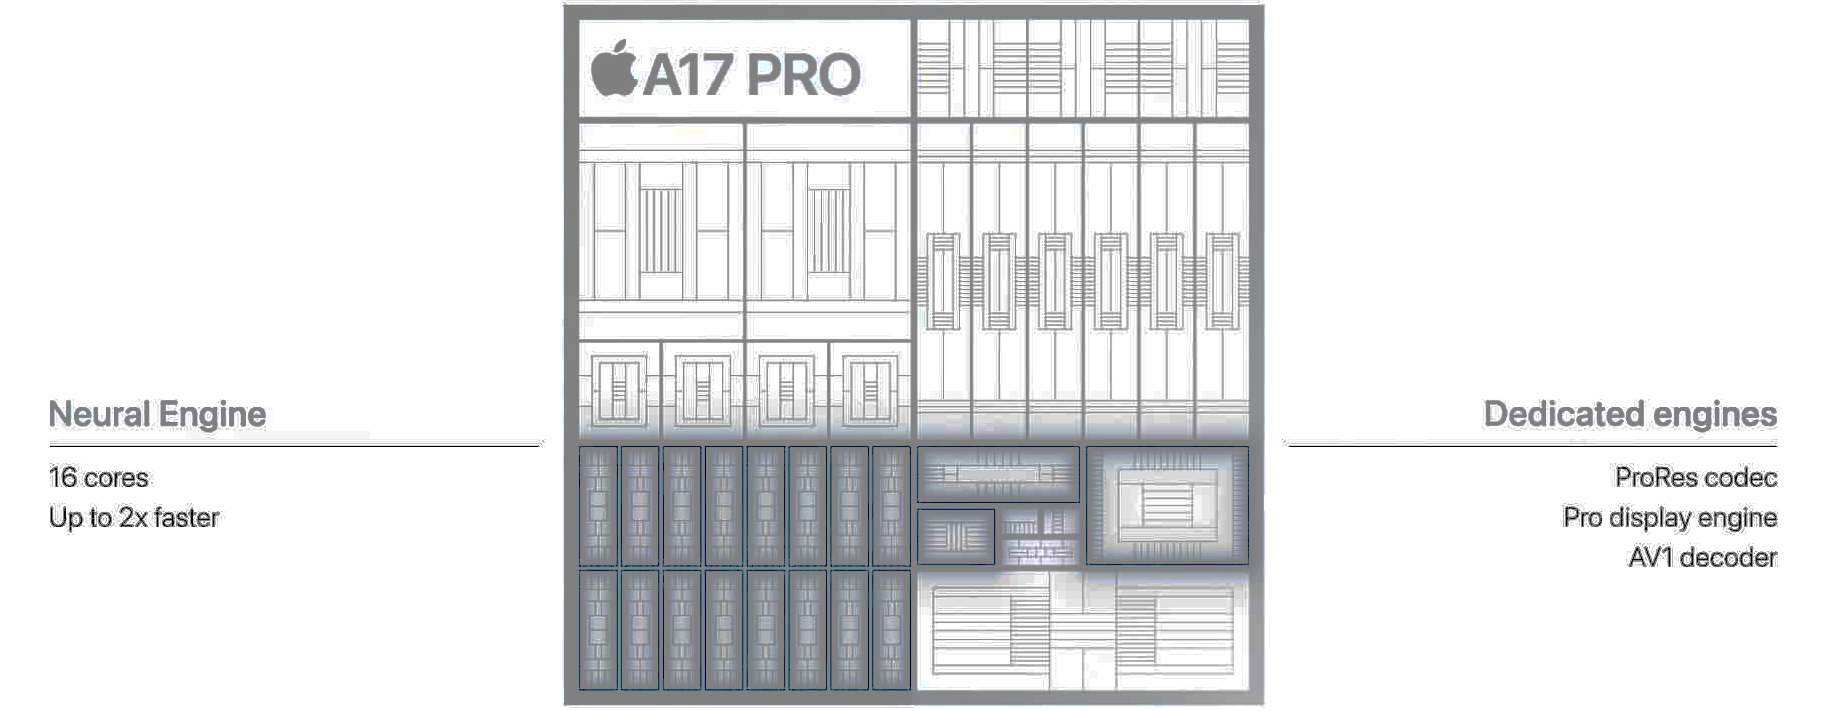
\includegraphics[width=1.1\textwidth]{./images/Apple_A17_Chip2.png}
	\caption{Neural Engine in Apple A17 Pro Chip}
	\label{fig:Apple_A17_Chip2}
\end{figure}

\newpage % Page break after cover page
\section{\textbf{General Overview}}
\begin{enumerate}[label=\textbf{\arabic*.}]
    \item \textbf{Micro-architecture}
    \begin{itemize}
        
            \item Apple's Neural Engine, first introduced with the A11 chip, is a specialized micro-architecture within Apple Silicon (like the M1 and M2 chips) designed to accelerate machine learning tasks. It includes multiple cores optimized for tensor processing, designed to perform matrix multiplications efficiently. The Neural Engine is tightly integrated within Apple's SoCs, allowing fast memory access and low latency.
            \item The architecture emphasizes energy efficiency and performance balance for real-time AI tasks on mobile and desktop devices.
       
    \end{itemize}

    \item \textbf{Programming Model}
    \begin{itemize}
        
            \item Developers primarily program the Neural Engine using Apple’s Core ML framework, which enables high-level APIs for deploying machine learning models on Apple devices. Core ML automatically optimizes models to take advantage of the Neural Engine, CPU, and GPU, depending on task requirements.
            \item Core ML can import models trained in popular frameworks like TensorFlow or PyTorch, converting them into formats optimized for Apple's hardware.
        
    \end{itemize}

    \item \textbf{Type of Parallelism}
    \begin{itemize}
            \item The Neural Engine uses both data and task-level parallelism. The engine is composed of multiple cores that can handle parallel processing of tasks, which is especially beneficial for tasks like image processing and other real-time AI tasks on-device.
            \item Apple's design is optimized for low-power parallel processing, making it ideal for mobile applications where energy efficiency is crucial.
    \end{itemize}

    \item \textbf{Comparison with Google’s TPU}
    \begin{itemize}
        \item \textbf{Micro-architecture Comparison:}
        \begin{itemize}
            \item Apple's NPU is designed for low-power, on-device computations, making it suitable for mobile and desktop AI applications. In contrast, Google’s TPU is designed for high-performance, high-throughput tasks in a data center environment, focusing less on power efficiency and more on computation speed.
        \end{itemize}
        
        \item \textbf{Programming Differences:}
        \begin{itemize}
            \item Apple's Neural Engine uses Core ML for programming, aiming to make machine learning integration seamless for developers on Apple platforms. Google's TPU, on the other hand, is closely integrated with TensorFlow, requiring a more specialized setup in Google’s ecosystem.
        \end{itemize}
        
        \item \textbf{Parallelism and Optimization:}
        \begin{itemize}
            \item While both employ parallelism, Apple's Neural Engine is optimized for task-level parallelism and energy efficiency, making it suitable for real-time applications on personal devices. Google’s TPU focuses on high-throughput data parallelism, suitable for large-scale neural network training.
        \end{itemize}
        
        \item \textbf{Use Case Differences:}
        \begin{itemize}
            \item Apple's NPU is aimed at enhancing AI-driven features on personal devices (like photo processing, augmented reality, and voice recognition), while Google’s TPU is intended for large-scale AI model training and inference in data centers, particularly for tasks that require extensive computational power without strict power constraints.
        \end{itemize}
    \end{itemize}
\end{enumerate}

\section*{Summary}
Apple’s Neural Engine and Google’s TPU serve distinct purposes. Apple’s NPU is optimized for on-device, energy-efficient processing for user-facing applications, while Google’s TPU is designed for large-scale AI processing in cloud environments where power constraints are less critical \cite{OpenAI}.

\bibliographystyle{IEEEtran} % or any other style you prefer
\bibliography{references}    % references.bib is the name of the .bib file
\end{document}
